\section{Propagation of Light in Three-level Atoms}
  \label{sec:nonlinear_threelevel}

    The solutions to the Maxwell-Bloch equations we have considered thus far
    have all involved the two-level atom model. In reality atoms consist of an
    infinite number of discrete levels along with a continuum of levels
    corresponding to the free electron. Two-level atom do not exist, but the
    model can successfully describe the interaction of a monochromatic field
    with a frequency near resonant with a pair of discrete energy levels. For
    multi-chromatic fields, other energy levels may need to be introduced due to
    transitions involving them becoming near-resonant with components of the
    field.

    The simplest extension of the two-level model is obviously to add a second
    frequency complement near-resonant with a third atomic level. This extension
    may seem incremental but in fact produces a variety of interesting and
    useful phenomena, due to the presence of quantum superposition dark states.
    Such phenomena include stimulated Raman adiabatic passage
    (\textsc{stirap})\cite{Grigoryan2001,Unanyan1998}, lasing without
    inversion\cite{Blok1990,Imamoglu1989,Scully1989} and
    phaseonium\cite{Scully1991,Eberly1996}, which have been well-studied in
    theory and experiment. We will discuss further two other well-studied
    phenomena in this thesis: matched pulses and simultons in this chapter, and
    electromagnetically induced transparency (\textsc{eit}) in chapter
    \ref{chp:polaritons}.

    \begin{figure}[]
      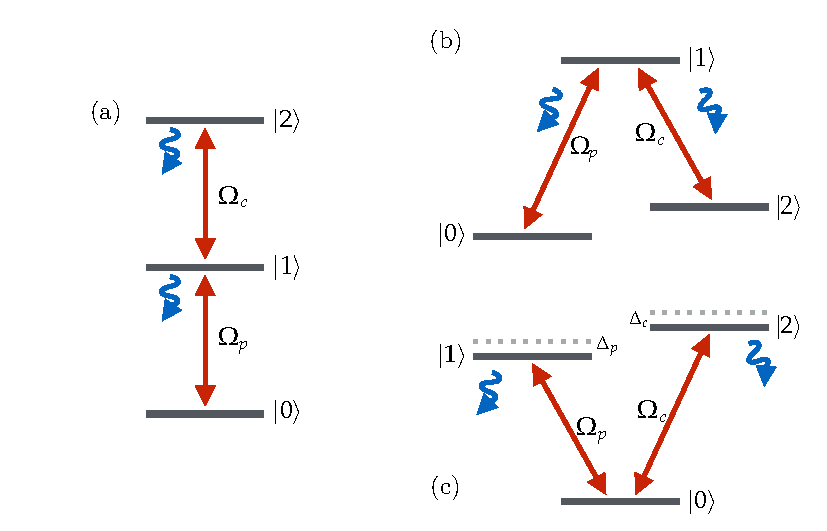
\includegraphics[width=\linewidth]
        {figs/03_nonlinear/three_level_diagrams_2.pdf}
      \caption{
      The three possible configurations of three-level atoms: (a) the $\Xi$ (or
      ladder) configuration, (b) the $\Lambda$ configuration and (c) the V
      configuration.
      }
      \label{fig:three_level_diagrams}
    \end{figure}

    First we take the opportunity to note that there are three available
    configurations of three-level atoms according to the transitions chosen for
    coupling. These are illustrated in figure \ref{fig:three_level_diagrams}.

    In the $\Xi$ (or ladder) configuration, the ground-state $\Ket{0}$ is
    coupled to the excited state $\Ket{1}$ as in the two-level atom, and a
    second field couples the transition from this intermediate excited state to
    a higher state, which we label $\Ket{2}$. The transition $\Ket{0}$ to
    $\Ket{2}$ is considered to be dipole forbidden by virtue of these states
    having the same parity. This configuration has probed useful for excitation
    to highly excited Rydberg states which allow for strong dipole-dipole
    interaction between atoms.\cite{Pritchard2010}

    In the $\Lambda$ configuration, the atom has two lower states $\Ket{0}$ and
    $\Ket{2}$, and a single excited state $\Ket{1}$ which is coupled to both
    lower states. These could for example represent a ground state hyperfine
    doublet. Coupling of the two lower states is taken to be dipole forbidden.
    We will investigate the $\Lambda$ configuration in greater detail when we
    investigate \textsc{eit} and the propagation of dark state polaritons in
    chapter \ref{chp:polaritons}.

    Finally, in the V configuration, the atom has two excited states $\Ket{1}$
    and $\Ket{2}$, and a single ground state level $\Ket{0}$ which is coupled to
    both excited states. We do not allow transitions between the two excited
    states. It is the V configuration we will consider further in this chapter,
    as we extend the theory of \textsc{sit} in two-level atoms to a pair of
    fields interacting with a thermal medium on resonance with transitions such
    that we describe the medium as consisting of V-type atoms.
